\documentclass[conference]{IEEEtran}
\usepackage{amsmath,amssymb,booktabs,graphicx,xcolor}
\usepackage[hidelinks]{hyperref}
\usepackage{url}
\usepackage{balance}
\usepackage{iftex}
\ifXeTeX
\usepackage{fontspec}
\setmainfont{texgyretermes-regular.otf}[BoldFont=texgyretermes-bold.otf,ItalicFont=texgyretermes-italic.otf,BoldItalicFont=texgyretermes-bolditalic.otf]
\setsansfont{texgyreheros-regular.otf}[BoldFont=texgyreheros-bold.otf,ItalicFont=texgyreheros-italic.otf]
\setmonofont{texgyrecursor-regular.otf}[BoldFont=texgyrecursor-bold.otf]
\fi
\definecolor{forest}{RGB}{32,75,64}
\title{Maintaining Source-Linked Evidence Views for Agent Memory}
\author{}
\begin{document}
\maketitle
\begin{abstract}
An agent's context combines records that cost different numbers of tokens and may outlive the repository state they describe. We demonstrate source-linked SQLite views for execution traces and code edits. One assembles tool evidence under a token budget and explains when an exclusion changes the optimal packet. The other tracks previously read code through editor-confirmed changes and checks displayed coordinates against file contents. On ISETrace a learned selector attained 83.07\% full evidence support against 81.19\% for first-fit on the same native ranking. On 1,071 code edits from 13 held-out issues, range-level invalidation preserved 302 complete packets against two under file-level invalidation. Matching unchanged lines within the editor arguments raised this to 323 without reading the file. All 25,912 retained lines checked on the edited paths matched their subsequent file snapshots. Halfway through the event history, our first-fit graph reader recovered 84.73\% complete support against 81.38\% for the stronger native graph reader. Visitors can exclude a dependency, relocate a surviving block and inspect incorrect source coordinates.

\end{abstract}

\section{Why maintain the evidence packet?}

A tool invocation and its result can reside in different trace events. A later decision may require both, within a limited context budget. When a source becomes unavailable, the system must decide whether the old selection is still valid. Even an unselected candidate can affect this decision.

In the demo, excluding a tool call replaces unit 11 with unit 19 at the same token cost and annotated coverage. Excluding a source outside the materialized dependencies avoids the optimizer entirely.

Wang et al.\ use execution provenance and relational graph models to retrieve supporting spans \cite{wang}. Bala examines which evidence survives packing \cite{bala}. Feng et al.\ study evidence needed in an observed coding-agent state \cite{feng}. MemTrace anchors immutable coding-agent traces to file, symbol and test identities and validates evidence before restoring it \cite{memtrace}. PACMI propagates validity changes through typed memory dependencies \cite{pacmi}. Qiu and Chen coordinate reads across stores using snapshots or epoch validation to deliver revision-consistent evidence \cite{readboundaries}. Given a coherent snapshot and its exclusions, our question is whether its \emph{optimal budgeted packet} survives unchanged.

Yi et al.\ retain extra ranked tuples to reduce refills in materialized top-$k$ views \cite{topk}. Here a cumulative-cost prefix constrains a second optimization. TAPE demonstrates temporal graph memory for personal agents \cite{tape}. Our visitor inspects which provenance dependencies suffice to reuse this two-stage selection. Runtime work on evolving coding-agent state tracks which observations remain current \cite{execledger}. We additionally track when a valid observation can change the bounded answer.

\begin{figure}[t]
\centering
\setlength{\fboxsep}{4pt}
\begin{tabular}{@{}c@{}}
\fcolorbox{forest}{white}{\parbox{.88\columnwidth}{\centering \textbf{Public execution trace}\\Events, argument/output fields and character offsets}}\\
$\downarrow$\\
\fcolorbox{forest}{white}{\parbox{.88\columnwidth}{\centering \textbf{Read-only SQLite projection}\\Unit, source span, directed relation, cost, rank, utility}}\\
$\downarrow$\\
\fcolorbox{forest}{white}{\parbox{.88\columnwidth}{\centering \textbf{Materialized view and source dependencies}\\Protected prefix, packed suffix and prefix boundary}}\\
$\downarrow$\\
\fcolorbox{forest}{white}{\parbox{.88\columnwidth}{\centering \textbf{Live visitor controls}\\Exclude a source, inspect a unit, compare maintenance plans}}\\
\end{tabular}
\caption{Serving architecture. A separate evaluator receives the resulting unit IDs and compares their source intervals with a private annotation table on demand. The selection path has no access to that table or to the bodies of tool calls.}
\label{fig:system}
\end{figure}

\section{Selection and source dependencies}

\subsection{Materializing a view}
For a query $q$, the input is an ordered set of candidates. Unit $i$ has token cost $c_i\geq 0$, learned utility $u_i$ and one or more source intervals. An interval identifies an event, a JSON field and a half-open range of character offsets. Several units can refer to the same source. Their selected token costs add even if their source intervals overlap. Evaluation later merges overlapping intervals in source coordinates to avoid double counting support.

Let $B$ be the token budget and $T\leq B$ the prefix threshold. Protect the longest consecutive prefix $H$ costing at most $T$; the first candidate outside $H$ is its boundary. The first-fit comparator scans the entire ranking, admitting any candidate that still fits.

A gradient-boosted tree estimates candidate membership in the annotated evidence from graph and dense rank, type, cost, graph score and gap to the leader, and pool size. We fit it on 3,894 training queries weighted equally and transform its log-odds into positive utility with softplus. Joint sufficiency is measured separately on held-out queries.

Write $C=B-\sum_{i\in H} c_i$. On the remaining candidates the selector maximizes $\sum_i u_i x_i$ subject to $\sum_i c_i x_i\leq C$ and $x_i\in\{0,1\}$. A standard exact dynamic program updates the value at each integer capacity. An explicit tie rule keeps the existing solution when a later candidate gives the same value. Selected IDs are returned in their original rank order. Threshold selection on 580 validation queries gave $T=1,024$ at $B=2,048$. Other thresholds trade a larger fixed prefix against additional freedom for the optimizer. The contribution here is a materialized packet with auditable source dependencies and maintenance rules.

\subsection{When can an exclusion change a packet?}
Let $P$ denote the stored packet and $D$ the set of candidate IDs removed by one or more source exclusions. Surviving candidates retain their order, costs and utilities. The budget, threshold and deterministic preference among tied solutions also stay fixed. Let $H'$ be the protected prefix recomputed on the remaining candidates.

\textbf{Reuse criterion.} The ordered packet is unchanged exactly when
\[
           D\cap P=\varnothing \quad\text{and}\quad H'\subseteq P.
\]
If a selected unit is removed, its ID cannot survive. If the new prefix contains a previously unselected unit, the new packet must contain that unit. For sufficiency, the first condition implies that all members of $H$ survive. Deletions can extend this prefix, so $H\subseteq H'$. By the second condition the old optimum contains every newly mandatory unit and remains feasible. Every packet feasible under the new requirement was already feasible before deletion. On these nested feasible families a previous optimum remains optimal, and the stable tie rule preserves its identity. Rank order of the surviving units is unchanged, giving equality of the ordered packets. The proof assumes exact comparisons and a stable tie order. A signed 64-bit implementation with fixed-point Q32 utilities reproduced all 10,000 original packets and all 108,204 deletion outcomes. The maximum tested utility sum was 13,789,213,370. Arbitrary floating-point summation orders do not inherit this guarantee.

A faster sufficient certificate indexes all sources of selected units and of the boundary. If an exclusion touches none of them, the old prefix survives and the suffix loses only unselected candidates. An index hit triggers recomputation, including some cases where the exact criterion would allow reuse.

A four-unit example illustrates the boundary. Let the budget be 8, the prefix threshold 4, costs $(3,3,1,5)$ and utilities $(1,1,3,10)$. The original prefix contains only unit 0 and the suffix chooses unit 3. Deleting unselected unit 1 forces the new prefix $(0,2)$. Only 4 tokens remain and unit 3 no longer fits. Monitoring only the chosen IDs would incorrectly return $(0,3)$.

\section{Implementation and visitor interaction}

The trace service uses SQLite tables for query-local units, cost, rank and utility, source intervals, and typed directed edges. A parameterized anti-join removes units incident on an excluded source. The interface traces each selected unit back to its event.

The trace projection has 5,009 units, 2,528 query-source pairs and 10,789 typed edges across 40 queries from distinct trajectories, sampled in a fixed hash order. ISETrace records real tool executions for synthetic OS-agent tasks \cite{ise,wang}. Its source exclusions are simulated. A second SQLite projection contains three actual coding-agent edits from Handoff Debt \cite{handoff}, selected to illustrate different outcomes. Its serving table holds block costs and observed ranges. A separate database holds file-snapshot witnesses. The consoles operate locally on anonymized metadata.

\begin{figure*}[t]
\centering
\begin{minipage}[t]{.48\textwidth}\vspace{0pt}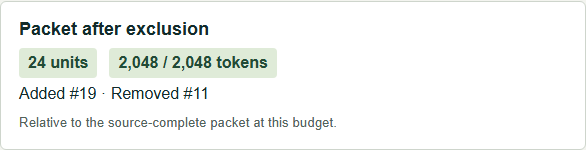
\includegraphics[width=\linewidth]{trace.png}\end{minipage}\hfill
\begin{minipage}[t]{.48\textwidth}\vspace{0pt}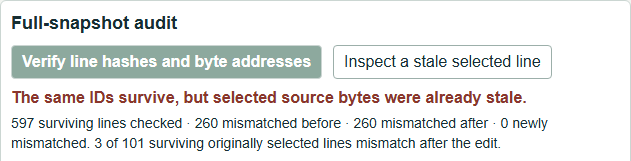
\includegraphics[width=\linewidth]{edit.png}\end{minipage}
\caption{Two running consoles. Left, excluding an execution source replaces unit 11 with unit 19 at the same cost. Right, a coding-agent edit retains the selected block IDs, yet the snapshot check detects incorrect line addresses in the original display. The audit operates separately from selection.}
\label{fig:ui}
\end{figure*}

\subsection{Visitor scenarios}
\textit{Change the trace evidence.} Select q02 and inspect a unit's source ranges. Exclude an unused source to reuse its packet, then exclude the selected source. Unit 19 replaces unit 11. Comparing the maintained result with full recomputation checks the ordered IDs. A separate evaluation control then shows that all 60 annotated characters remain covered.

\textit{Change the budget or boundary.} Reduce the token budget and inspect which supporting range drops out. In q07 an exclusion touches only the indexed prefix boundary. The conservative plan recomputes, while the exact test establishes that the packet survives.

\textit{Follow a real code edit.} Switch to the edit console and choose a recorded case. In the first, a line shift preserves a 315-byte packet and its two block IDs. In the second, the edit intersects two of three blocks, leaving 74 of 507 bytes. In the third, all 14 IDs and 2,044 bytes survive. Auditing the underlying snapshots identifies three selected lines whose reported addresses were already wrong before the edit. Each outcome is a recorded example; the larger evaluation below estimates their prevalence on its stated cohort.

\textit{Reuse context from the edit itself.} The Edit Context console exposes the old and replacement line fingerprints. Choose the interior-lines example. Range invalidation drops both original blocks, matching the ends recovers one, and aligning equal runs restores both. The visitor changes the rule or byte budget and verifies the resulting coordinates against independently stored witnesses.

\section{Measurements and interpretation}
\subsection{Budgeted evidence recovery}
ISETrace provides 2,000 held-out queries over 1,207 trajectories. Its Full Support metric equals one when selected intervals jointly cover every annotated source interval. We use matched candidate units, token costs and five shared retrieval seeds. In the first-fit control, skipped items leave their budget available for later candidates.

\begin{table}[t]
\caption{Evidence recovery under a 2,048-token cap. Values are means across five matched seeds on the complete test.}
\centering\small
\begin{tabular}{lrr}\toprule
Selector & Support (\%) & Tokens/query\\\midrule
Full R-GCN, strict prefix & 78.60 & 1,854.95\\
No adjacency, strict prefix & 79.21 & 1,850.31\\
Full R-GCN, first-fit & 80.44 & 2,039.97\\
No adjacency, first-fit & 81.19 & 2,039.83\\\midrule
Dense order + exact packing & 75.25 & 2,038.61\\
Graph rank-weighted packing & 80.37 & 2,036.40\\
Graph utility/cost greedy & 82.31 & 2,034.63\\
Same-ranker first-fit & 82.19 & 2,039.30\\
Prefix + exact packing & 82.60 & 2,039.12\\
No adjacency + learned packing & 83.07 & 2,039.12\\
\bottomrule\end{tabular}
\label{tab:retrieval}
\end{table}

Wang et al. report 77.33\% Full Support for the residual R-GCN in their main table \cite{wang}. Our controlled comparisons use local retraining of both native configurations. The full native relational graph model and its separately trained ablation without chunk adjacency are paired by seed, query, candidate set and cost. Our primary graph ordering with learned packing reaches 82.60\%, versus 82.19\% for its own first-fit (difference $+0.41$ points, crossed 95\% interval $[-0.23,1.08]$). Over six budgets from 256 to 8,192 tokens, normalized Full Support AUC is 70.992\% versus 70.565\% ($+0.427$ points, $[0.102,0.758]$).

The strongest tested hybrid uses the no-adjacency model's prefix and our learned utility. Against first-fit on that same native ranking, it gains 1.88 points ($[0.76,3.07]$) at 2,048 tokens. We selected this ordering after inspecting the budget curves. Sorting by absolute learned utility is a strong inexpensive alternative: its AUC is 71.204\%, against 71.324\% for exact packing ($+0.120$ points, $[-0.053,0.298]$). The trace console uses the primary 82.60\% configuration. All quoted retrieval measures concern evidence availability under a fixed cap.

At the halfway checkpoint we rebuilt graphs from truncated raw histories. On 901 questions in 657 trajectories with all evidence already present, our ranking with first-fit reached 84.73\%, dense first-fit 77.25\%, and the stronger native no-adjacency model 81.38\% ($+3.35$ points over native, $[1.40,5.35]$). All used approximately 2,014 tokens. Filtering completed native rankings to visible candidates gave 84.24\%, overstating the actual baseline by 2.86 points ($[1.59,4.24]$). Reciprocal rank fusion reached 85.50\% ($+0.78$ over our rank, $[-0.54,2.09]$). On all 2,000 questions, including unavailable evidence, our rank, the native comparator and their fusion attained 40.65\%, 39.01\% and 40.98\%, respectively. Query times are simulated.

What contributed beyond position and recency? Holding the training set, boosting model, E5 scores, token costs, event metadata and selector fixed, adding typed graph-degree features raised Full Support from 79.16\% to 83.57\% ($+4.42$ points, $[2.79,6.09]$). Adding cross-event relations to a reader that already had local relations gained 4.17 points ($[2.57,5.83]$). Local relations alone added 0.24 points to metadata ($[-0.60,1.12]$). Permuting the assignment of degree vectors within each role reduced support to 78.89\%. These are controlled feature comparisons on the same halfway panel.


\subsection{View maintenance on a live projection}
On 40 frozen-model projections, the portable reader reproduced every ordered packet at 2,048 tokens. Independent interval arithmetic matched the official metric. Mean size was 2,043 tokens and 36 packets had complete support.

We independently excluded each of the 2,528 query-source pairs from the initial snapshot. The indexed sufficient certificate served the old packet on 2,041 exclusions and recomputed the remaining 487. Ordered IDs matched fresh recomputation on every operation. Three conservative recalculations left the packet unchanged. The cache-hit rate was 80.74\% across exclusions and 77.80\% when each trace was weighted equally.

Both plans used identical SQLite data, native packing and precomputed features. Three interleaved repetitions gave 7,584 timed executions per plan. Aggregate full-recomputation time divided by certificate time was $5.16\times$, with a 95\% trajectory-bootstrap interval of $[4.36,6.17]$. Median latency fell from 280.25 to 9.30 microseconds and p95 from 540.29 to 352.82 microseconds. The dependency index added a mean 116 microseconds of setup per query. These are warm, single-host serving measurements. They exclude model training, feature extraction, browser rendering and evidence evaluation. The interactive portable implementation uses a Python optimizer to make the same decisions without native dependencies.

\balance
\begin{table}[t]
\caption{Exact reuse under independent hypothetical source exclusions. The final column counts additional reuse approvals beyond the fast boundary certificate.}
\centering\small
\begin{tabular}{rrrr}\toprule
Sources removed & Cases & Unchanged & Additional\\\midrule
1 & 2,528 & 2,044 & 3\\
2 & 97,676 & 68,336 & 232\\
3 & 4,000 & 1,991 & 12\\
8 & 4,000 & 890 & 17\\
\bottomrule\end{tabular}
\label{tab:exclusions}
\end{table}

Across 108,204 source-deletion sets (Table~\ref{tab:exclusions}), the exact criterion identified all 73,261 unchanged packets and certified 264 more reuses than the conservative index. Exhaustive checks of 20,204 deletion sets on 320 small synthetic pools also passed, including ties. These results assume fixed scores, costs, rank and budget. The timed speedup concerns the conservative single-source plan.

\section{Serving memory during code edits}
We replayed 3,525 observed write attempts from Handoff Debt~\cite{handoff} on 37 issues across five Python repositories. Windows were selected around an observed read followed by a confirmed replacement. A separate integer view packs recent line blocks under a 2,048-byte cap. Whole-file invalidation permitted reuse in six of 2,820 attempts affecting a present path. Invalidation granularity and workload therefore matter to the benefit of caching.

A receipt locates the changed lines. We invalidate overlapping blocks and shift surviving addresses. A guard withholds displayed suffixes after clipping or coordinate discontinuities. Frozen on 24 issues, it retained 43,299 of 47,924 candidate lines on the other 13. Across 1,071 edits, range maintenance preserved 302 complete packets, versus 2 for file invalidation, 92 for symbol invalidation using Python syntax trees, and 287 for unique content matching against the new file. Issue-macro gains were 26.14 points over files ($[19.70,32.23]$), 17.92 over symbols ($[12.73,23.01]$) and 1.56 over content ($[-2.19,5.39]$). Content matching retained more individual bytes. All 25,912 surviving lines checked on edited paths matched their subsequent snapshots. A coding-task success gain remains unestablished.

An editor replacement also supplies two literal strings. We compare boundary-tagged line fingerprints, anchor their common ends and align unchanged interior runs within a bounded edit window. A block survives if every line maps to a consecutive equal line. Using just the common ends preserved 322 packets, and adding the interior alignment preserved 323 ($+1.97$ issue-macro points over range invalidation, $[1.02,3.03]$). We audited all 29,713 mapped lines on the edited paths. Across these operations the literals totalled 1.22 MB, versus 141.18 MB for pairs of complete file versions. A backend with version access can combine range validation with unique content lookup for intersecting blocks: it preserved 341 packets ($+4.52$ points over unique lookup alone, $[2.13,7.41]$).

Packet stability does not establish subsequent use. We followed requests until the next edit, termination or loss of observability. On this cohort 69 informative reads occurred in 54 observable episodes, with 889 right-censored windows. Range validation and local alignment supplied evidence beyond the edit receipt in the same 13 episodes. They fully covered 4 and 6 of these reads, respectively, when combined with the receipt. On a separate public SWE-agent run with Claude 4 Sonnet~\cite{swe-run}, we excluded all tasks shared with Handoff Debt. Across 265 eligible edits from 159 SWE-bench Verified issues, local alignment preserved 7 packets versus 5 for ranges ($+0.75$ issue-macro points, $[0.00,2.14]$). Source localization succeeded for 178 edits. This transfer is inconclusive. These observations do not establish a solver-level gain.

On 40 ISETrace projections we also replayed arrivals at the original message positions. Caching the optimal suffix for each capacity and updating it after new units gave exactly the full solution at all 2,336 steps and reduced selector time by $3.88\times$ ($[3.16,4.83]$) on one CPU. This separate operator study fixes costs, ranks and utilities throughout each replay; it excludes encoder and graph-scoring time. The visitor scenarios expose packet identity, source validity and the cost of maintaining each.

\section*{Acknowledgments}
OpenAI Codex assisted with the design and implementation of the methods in Sections II and III, experimental pipelines and analyses in Sections IV and V, preparation of the figures and demonstration, and drafting of the manuscript. Reported measurements were computed by the cited evaluation code and checked against persisted per-query or per-edit results.

\bibliographystyle{IEEEtran}
\bibliography{sources}
\end{document}
